%%%% Proceedings format for most of ACM conferences (with the exceptions listed below) and all ICPS volumes.
\documentclass[sigconf]{acmart}
%%%% As of March 2017, [siggraph] is no longer used. Please use sigconf (above) for SIGGRAPH conferences.

%%%% Proceedings format for SIGPLAN conferences 
% \documentclass[sigplan, anonymous, review]{acmart}

%%%% Proceedings format for SIGCHI conferences
% \documentclass[sigchi, review]{acmart}

%%%% To use the SIGCHI extended abstract template, please visit
% https://www.overleaf.com/read/zzzfqvkmrfzn


\usepackage{booktabs} % For formal tables


% Copyright
%\setcopyright{none}
%\setcopyright{acmcopyright}
%\setcopyright{acmlicensed}
\setcopyright{rightsretained}
%\setcopyright{usgov}
%\setcopyright{usgovmixed}
%\setcopyright{cagov}
%\setcopyright{cagovmixed}
\usepackage[ampersand]{easylist}
\usepackage{amssymb}
\usepackage{multicol}
\usepackage{multirow}

% DOI
\acmDOI{10.475/123_4}

% ISBN
\acmISBN{123-4567-24-567/08/06}

%Conference
\acmConference[CHASE'18]{11th International Workshop on Cooperative and Human Aspects of Software Engineering}{May 27, 2018}{Gothenburg, Sweden} 
\acmYear{2018}
\copyrightyear{2018}


\acmArticle{4}
\acmPrice{15.00}

% These commands are optional
%\acmBooktitle{Transactions of the ACM Woodstock conference}
%\editor{Jennifer B. Sartor}
%\editor{Theo D'Hondt}
%\editor{Wolfgang De Meuter}

\newif\ifdraft
\drafttrue

\newcommand{\boldification}[1]{\ifdraft\indent\textbf{#1}\\\indent\else\relax\fi}



\begin{document}
\title{Context in Programming: An investigation of how developers create context}
% \titlenote{Produces the permission block, and copyright information}
% \subtitle{Extended Abstract}
% \subtitlenote{The full version of the author's guide is available as
%   \texttt{acmart.pdf} document}


% \author{Ben Trovato}
% \authornote{Dr.~Trovato insisted his name be first.}
% \orcid{1234-5678-9012}
% \affiliation{%
%   \institution{Institute for Clarity in Documentation}
%   \streetaddress{P.O. Box 1212}
%   \city{Dublin} 
%   \state{Ohio} 
%   \postcode{43017-6221}
% }
% \email{trovato@corporation.com}

% \author{G.K.M. Tobin}
% \authornote{The secretary disavows any knowledge of this author's actions.}
% \affiliation{%
%   \institution{Institute for Clarity in Documentation}
%   \streetaddress{P.O. Box 1212}
%   \city{Dublin} 
%   \state{Ohio} 
%   \postcode{43017-6221}
% }
% \email{webmaster@marysville-ohio.com}

% \author{Lars Th{\o}rv{\"a}ld}
% \authornote{This author is the
%   one who did all the really hard work.}
% \affiliation{%
%   \institution{The Th{\o}rv{\"a}ld Group}
%   \streetaddress{1 Th{\o}rv{\"a}ld Circle}
%   \city{Hekla} 
%   \country{Iceland}}
% \email{larst@affiliation.org}

% \author{Valerie B\'eranger}
% \affiliation{%
%   \institution{Inria Paris-Rocquencourt}
%   \city{Rocquencourt}
%   \country{France}
% }
% \author{Aparna Patel} 
% \affiliation{%
%  \institution{Rajiv Gandhi University}
%  \streetaddress{Rono-Hills}
%  \city{Doimukh} 
%  \state{Arunachal Pradesh}
%  \country{India}}
% \author{Huifen Chan}
% \affiliation{%
%   \institution{Tsinghua University}
%   \streetaddress{30 Shuangqing Rd}
%   \city{Haidian Qu} 
%   \state{Beijing Shi}
%   \country{China}
% }

% \author{Charles Palmer}
% \affiliation{%
%   \institution{Palmer Research Laboratories}
%   \streetaddress{8600 Datapoint Drive}
%   \city{San Antonio}
%   \state{Texas} 
%   \postcode{78229}}
% \email{cpalmer@prl.com}

% \author{John Smith}
% \affiliation{\institution{The Th{\o}rv{\"a}ld Group}}
% \email{jsmith@affiliation.org}

% \author{Julius P.~Kumquat}
% \affiliation{\institution{The Kumquat Consortium}}
% \email{jpkumquat@consortium.net}

% The default list of authors is too long for headers.
\renewcommand{\shortauthors}{S. Chattopadhyay et al.}


\begin{abstract}
This paper provides a sample of a \LaTeX\ document which conforms,
somewhat loosely, to the formatting guidelines for
ACM SIG Proceedings.\footnote{This is an abstract footnote}
\end{abstract}

%
% The code below should be generated by the tool at
% http://dl.acm.org/ccs.cfm
% Please copy and paste the code instead of the example below. 
%
\begin{CCSXML}
<ccs2012>
<concept>
<concept_id>10003120.10003121.10003126</concept_id>
<concept_desc>Human-centered computing~HCI theory, concepts and models</concept_desc>
<concept_significance>300</concept_significance>
</concept>
<concept>
<concept_id>10003120.10003121.10011748</concept_id>
<concept_desc>Human-centered computing~Empirical studies in HCI</concept_desc>
<concept_significance>300</concept_significance>
</concept>
<concept>
<concept_id>10003120.10003130.10003131</concept_id>
<concept_desc>Human-centered computing~Collaborative and social computing theory, concepts and paradigms</concept_desc>
<concept_significance>300</concept_significance>
</concept>
</ccs2012>
\end{CCSXML}

\ccsdesc[300]{Human-centered computing~HCI theory, concepts and models}
\ccsdesc[300]{Human-centered computing~Empirical studies in HCI}
\ccsdesc[300]{Human-centered computing~Collaborative and social computing theory, concepts and paradigms}


\keywords{Context definitions, psychology of programming}


\maketitle

%!TEX root = main.tex

\section{Introduction}

\boldification{Context is <any pertinent information that is needed to complete a task>. We all, including developers intuitively know this. To help developers in their programming tasks, understanding how developers build and maintain context is important. }

\boldification{However, it is hard to have an operational definition of context, over the years two schools of thoughts have evolved -- representational and interactional}

\boldification{Representational view looks at context as tangible, delineable and stable. Researchers have adapted this view in SE by operationalizing it as context represented as artifacts, tasks or environmental factors**...But it misses this}

\boldification{However, this still leaves us with the question ``what is context?''. This leads to the view of context as an interactional problem originating from ubiquitous computing}

\boldification{Interactional view defines context as a relational property that holds between objects or activities and focuses on the dynamic nature of context}

\boldification{However, although more intuitively accurate, this is more difficult to operationalize. In this paper we want to explore how observing interactions of a programmer with artifacts within and outside the IDE and the process of solving a programming task can help us gain insight about how context is created and evolved}

Programming, in particular the act of coding, does not occur in isolation. It involves ideating and exploring different solutions and using different types of information (in the codebase and from on-line/external resources) to complete a task. These relevant pieces of information, along with the programmer's prior knowledge, creates a context that the programmer uses to solve the task.  


%These varied pieces of information and solutions that the programmer explored to complete the task along with the knowledge that she already possessed creates the context for solving the programming task. ------- re-framed above---------

%Modeling this programming context is difficult as it not only involves the artifacts that were used, but also the specific information value of these artifacts, the  programming activity that guided the interaction with the artifact, and the mental mapping between the information found and the problem at hand. ---Moved to discussion---

In software engineering, `context' has been described as the perspective gained from all relevant information obtained from these different sources. Although we intuitively understand context; it is a ``slippery notion''~\cite{Dourish:2004}---hard to formally describe and define. It is dynamic in nature, morphing with every action and evolving along with changing goals. 

%One of the problems is that it is a concept that stays in the periphery while a developer completes a task, but slips away when someone attempts to precisely define it. The second problem is that context is continually renegotiated and redefined based on the current course of action and task goals. ------ re-framed----
Context has been researched in both software engineering and ubiquitous computing, resulting in two disparate views of context---representational and interactional context~\cite{Dourish:2004}.
% Over the years, research in ubiquitous computing has influenced the concept of `context' in software engineering. Paul Dourish recalls that this has resulted in two disparate views of context---representational and interactional context~\cite{Dourish:2004}.

The \textit{representational view} describes context as delineable and stable~\cite{Schilit:1994a,Abowd:1999,Pascoe:1998}. To operationalize this view, researchers have attempted to encode context through artifacts, tasks, and environmental factors. For example, Gasparic et al.~\cite{Gasparic:2017} discuss how context can be modeled by environmental factors like who is working, what is the environment, which artifacts are involved etc.
However, focusing only on how context is represented leaves gaps in our understanding of how context is created, how it is affected by developers' goals, and how it changes with evolving goals. 
% However, focus on representing context through factors still leaves the burning question `what is context?' Can context be defined as the sum of all these factors? Are there other elements that add to the context? Which of these factors are contained within the context? Which are the factors that only affect the context?

The \textit{interactional view} defines context as a relational property that exists between objects or activities; and one cannot be viewed disjointed from the other ~\cite{Dourish:2004}. Because of this interconnected relationship, contextual factors must be defined dynamically for each activity, and the sequence in which they occur is important.

In this paper, we present our study of six programmers and observations about how programmers create context by interacting with artifacts. Our (qualitative) analysis provides evidence that context crosscuts activities and artifacts, thereby calling the need for a merging of the representational and interactional views of context.

%we aim to understand how programmers create context: what role programming activities plays in creating context and how it guides interactions with the artifacts and the environment. We observed six programmers engaged in exploratory programming and (qualitatively) analyzed their programming behavior and interactions with artifacts. 

%We observed that interactions with the artifacts and the programming activity together guide programmers to find and obtain the information that shapes context. <<Add after results finalized>>
% Information, depends on interaction, can be represented activities and artifacts and the interaction between them.
% Our observations also indicate that context has representational factors, is defined by ???

% interactional processes, and is informational by nature. This warrants further studies to accurately model the context creation behavior of programmers.
%!TEX root = main.tex

\section{Related Work}

\boldification{Context is an foundational concept borrowed from Ubiquitous Computing. Many such research capture context along with information to for retrieval purposes [(Freeman and Gelernter 1996), Dourish2000] or to influence system behavior based on usage patterns[(Cheverst et al. 2000)]	}

\boldification{Authors like [Schillit and theimer, Brown, Ryan] define context in ?context-aware? computing domain as various factors of the user like location, time, identity etc.}

\boldification{More related to the software engineering field are the definitions provided by [Brown, Ward, Rodden] which capture context as factors of the user?s environment or application settings}

\boldification{Murphy has made extensive contribution to import ?context? into building better software by trying to capture various factors like programming task(Mylar), artifacts(Hipikat) and the state of the environment(Gasparic)}

\boldification{Such representational understanding of context is accurate for software systems, as softwares are inherently built to represent states. However, they only answer ?what can be used to represent context?? rather than ''what is context?''}

\boldification{[Pascoe] defines context as subset of physical and conceptual state of user. [Dey] takes the notion forward by introducing user?s emotion, attention and informational state as part of context. He points out that context can be seen as an interactional instead of representational}

\boldification{This view of context is hard to operationalize. Although Spyglass [Murphy and V\_porn] subscribed to this notion of context to implement an intuitive recommender, a model of context that accounts for interactions is missing}

\boldification{In this paper we take a look at if visualizing what developers do throws any light as to how programmers actually build context. Without prescribing to any particular view of context, we explore what processes shape the programmer?s perceived context}


%!TEX root = main.tex

\section{Methodology}\label{sec:methodology}

\boldification{We observed 5 participants at work. Out of these we chose 3 participants who represent diverse styles of programming. P1 followed Test driven development approach, P4 was a conscientious programmer and S was a tinkerer.}

We conducted a lab study where we observed six graduate students with professional programming experience perform a programming task. Their details are presented in Table ~\ref{tab:participant-demographics}.
We provided participants P1 through P5 with a prompt requiring planning, designing, and developing software to simulate a traffic intersection. We used this prompt as it has been used in prior studies~\cite{Mangano:2012}. We modified the prompt slightly requiring that participants develop at least parts of the software. This prompt was easy to understand, yet nontrivial to implement, allowing us to observe participants' use of context when programming.

We observed another participant P6 working on a real-world problem of developing his own IDE. We do so to contrast the results of participants who were working on a given prompt (and the specifics of that prompt) from those that occur when a programmer is working on their on own programming task.

% We observed P6 working on a real-world problem of developing his own IDE. Contrasting the results of P1-P5 with P6 allowed us to differentiate observations that arose due to the specifics of the traffic prompt, from those that occur during typical software development.

%!TEX root = ../main.tex

\begin{table}[!htbp]
%\vspace*{-0.8\baselineskip}
\caption{Participant Demographics}
\label{tab:participant-demographics}
\centering
\begin{tabularx}{0.47\textwidth}{CcRR}
\toprule
	\textbf{Participant} & \textbf{Gender} & \textbf{Programming \mbox{Language}}\parnote{Programming language selected by participant.} & \textbf{Programming Experience}\parnote{Programming experience across all programming languages.} \\
\midrule
	P1 & M & Scala & $>$10 yrs. \\
	P2 & M & C/C++ & 7 yrs. \\
	P3 & F & Python & 5 yrs. \\
	P4 & F & Java & 7 yrs. \\
	P5 & F & Python & $>$10 yrs. \\
	P6 & M & JavaScript & $>$10 yrs. \\
\bottomrule
\end{tabularx}
\parnotes
%\vspace*{-0.8\baselineskip}
\end{table}

%beyond the domain of ``toy systems''.
In this paper, we discuss our observations from P1, P4, and P6. This subset of participants represent a diverse set of programming styles; P1 adhered to the Test-Driven Development (TDD) model, P4 followed the Design-Driven Development (DDD) model, and P6 displayed a strong affinity for tinkering~\cite{Beckwith:2006}. %By focusing on these three participants we are able to better present context while programming. 

\boldification{P1 and P4 was given to design(or redesign?? Clarify from Nick) a traffic simulator application that would be used for educational purposes. This style of programming is similar to maintenance or debugging. P6 was working on developing an IDE, which was more exploratory in nature with just some idea about the work and lesser constraints.}

% P6 was not given a prompt because we wanted examine whether our initial observations from P1 to P5 would hold in a unconstrained real-world environment. This allowed us to differentiate observations that arose due to the specifics of the given traffic prompt, and those observations that appear to be universal across programming sessions and goals. The traffic prompt given to P1 to P5 is similar to a prompt use in previous software design studies~\cite{Mangano:2012}, and asks participants to design and implement a simulator for traffic intersections that can accommodate users experimenting with different timing and traffic light signal patterns. This prompt was designed to be easily understandable but difficult to implement, in order to challenge participants and be able to observe their use of context in problem solving. ------Moved up---------

\boldification{We captured their screen for an hour. P1 was asked to think aloud. We used his verbalizations to validate our understanding of context creation, usage and deletion}

We time-boxed the study to be one-hour long to prevent participant fatigue~\cite{Easterbrook:2008}. Participants used their preferred development tools for the study. They were also provided blank paper and given the option to think aloud; however, only P1 chose to think aloud. We used this think-aloud data to validate our interpretations of P1's actions. We used the diverse collection of data -- audio, screen recording, external notes -- to build our observations of how programmers create context.

% We used this think aloud data to validate our interpretations of participants' actions when programming. Context is a broad notion, and anything---from a paper note's placement to the screen color---can affect context. We obtained diverse data in the form of think aloud audio, screen recording video, facial expressions, and any external notes added to either the blank paper or the printed traffic intersection prompt. 

% We didn't restrict our observation to any medium, as context is a broad notion and anything around a person, from the placement of a paper to the color of the screen, can affect it. We also collected diverse data in the form or think aloud, screen capture, facial expression, video of workspace and any notes or diagrams the participants drew to recognize the subtle hints which may suggest that information was added to the context or obtained from the context. 

% Study sessions lasted time-boxed to a maximum of one hour, and organized as observational lab studies~\cite{Easterbrook:2008}. Participants were allowed to use their preferred development tools during the study, and video capture of their screen was recorded. Paper and pen were provided to participants for design, sketch, and note-taking purposes, and was collected at the conclusion of the study. Only P1 used a think-aloud, which was used to gain a better understanding of their mental model of context while problem solving.

\boldification{We unitized the videos using atlas.ti based on groups of coherent activities. For each unit, we noted the programming activities the participants performed and the artifacts they accesses and in what order. The set of programming activities were large adapted from [Yi wang?s] paper.}

%%% HOW TO EXPLAIN EPISODES WITHOUT EPISODES???????

To analyze the data, the first author single-handedly unitized the screen recordings into continuous time segments. Each unit contains a group of related interactions that participants made towards achieving a small part of their programming task. For example, a unit on analysis for participant P6 involved him working on a source code file, running the code, and assessing the output in the terminal. The first author also unitized all the transcripts.

For each of these units, we identified the programming activity, the artifacts used, and the frequency of use. Table ~\ref{tab:programming-activities} lists  the 12 programming activities we use in our analysis. The codeset builds on Yi Wang's~\cite{Wang:2017} activity codes, with slight modifications to fit our task prompt---we changed \texttt{READING QUESTIONS} to \texttt{[A4] READING TASK PROMPT}, and added \texttt{[A1] UPDATING DOCUMENTS} and \texttt{[A2] COMMUNICATING}.

Using this code set, the first and the third authors obtained an Inter-Rater Reliability (IRR) score of 97.14\% and the first and the fourth authors obtained an IRR score of 92\% when coding random segments from the selected participants dataset (which constituted \textasciitilde14\% of the raw data). The remaining 86\% of the data was coded individually by these three authors.

We identified the artifacts that participants used in these units. We categorized artifacts as web-pages, source code files open and visible on screen, and external notes. Example artifacts include \texttt{intersection.scala} open as a file, and \texttt{stackoverflow.com} visited in the browser. 
%Our codeset is based upon the codes developed by Yi Wang~\cite{Wang:2017}, which include: \texttt{navigation, reading questions, searching, reading search results, processing search results, viewing web resources, coding, run, debugging,} and \texttt{idle}. We do not use the \texttt{accidents} code since determining whether fast switching between artifacts is intentional, and therefore productive, is difficult to appraise from screen capture data. We added \texttt{communication} and \texttt{documentation} to the codeset, due to the nature of the tasks found in the traffic prompt and the think-aloud included in P1.

\boldification{Three of the authors coded the videos, following the IRR process. They obtained a jaccard index of 97.3\%. They also manually noted the order in which participants accessed the artifacts}



%!TEX root = main.tex

\section{Study Results}

%!TEX root = ../main.tex

\begin{table*}
\caption{Programming activities and the most frequently accessed artifacts associated with them}
\label{tab:programming-activities}
\begin{tabular}{lll}
\toprule
Programming Activity & Artifact type [frequency] & Artifact type frequencies for each type \\
\midrule
\multirow{3}{*}{A0 - Coding} & Code [32] & [2,6,5,4,12,2,1] \\
& Tools [12] & [1, 1,5,1,3,1] \\
& Documents [2] & [2] \\
\midrule
\multirow{2}{*}{A1 - Interaction with documents} & Documents [19] & [19] \\
& External Artifacts [20] & [13,7] \\
\midrule
\multirow{2}{*}{A2 - Navigation} & Code [9] & [0,1,1,0,5,1,1] \\
& Tool [1] & [0,0,1,0,0,0] \\
\midrule
\multirow{2}{*}{A4 - Reading Task Prompt} & Documents [22] & [22] \\
& External Artifacts [15] & [10,5] \\
\midrule
\multirow{2}{*}{A5 - Searching in web/IDE} & Code [4] & [0,0,1,1,2,0,0] \\
& Tool [1] & [0,0,1,0,0,0] \\
\midrule
\multirow{2}{*}{A6 - Reading Search Results} & Code [1] & [0,0,0,0,1,0,0] \\
& Web Resource & [1] \\
\midrule
\multirow{2}{*}{A7 - Processing Search Results} & Code [2] & [0,0,0,0,2,0,0] \\
& Web Resource & [1] \\
\midrule
\multirow{2}{*}{A8 - Viewing Web Resource} & Code [1] & [0,0,0,0,1,0,0] \\
& Web Resource & [1] \\
\midrule
A9 - Debugging & Code [1] & [0,0,0,0,1,0,0] \\
\midrule
\multirow{2}{*}{A11 - Idle} & Documents [2] & [2] \\
& External Artifacts & [1,1] \\
\bottomrule
\end{tabular}
\end{table*}

\begin{figure}
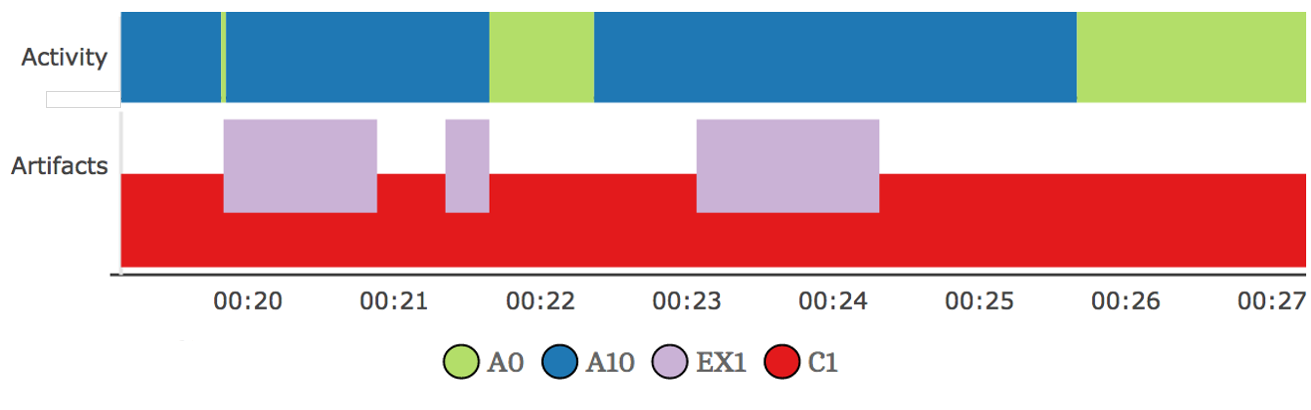
\includegraphics[width=\columnwidth]{figures/P1timeplot}
\caption{Snippet of Activities and Artifacts from P1(traffic intersection prompt, 8-minute duration)}
\label{P1Fig}
\end{figure}

\boldification{here we report on how participants created and used context as they were working on their programming task.}
In this paper, we investigate how people create context for programming tasks. We present the observations we draw from the participants' interactions with the artifacts during specific programming activities. Our focus was to develop an understanding of how the context building process occurs, and gain insights into which factors play a role in shaping context.


We observe the types of artifacts that participants refer to when performing different programming activity. The participants interacted with six different types of artifacts: \textit{source code files} (e.g. \texttt{intersection.js} and \texttt{car.java}), \textit{documents} (task prompt), \textit{IDE tools} (\textit{New Class} dialog box, getter-setter dialog boxes (e.g. \texttt{T2}), terminal/console),\textit{ web resources} (e.g. Google search results, Stack-Overflow pages, API documentations), \textit{externalized artifacts} (e.g. sticky notes, paper diagrams), and \textit{other} (e.g. calculators, project setup dialog boxes).

For our analysis purpose, for each participant, we will refer to the source code files as \texttt{C1}, \texttt{C2}, \ldots , etc., the document as \texttt{D1}, IDE tools as \texttt{T1}, \texttt{T2}, \ldots, etc., web resources as \texttt{W1}, \texttt{W2}, \ldots, etc., external artifacts as \texttt{EX1}, \texttt{EX2}, \ldots, etc., and other tools as \texttt{O1}, \texttt{O2}, \ldots, etc. The sequence of these tags depend on the sequence in which each participant encounters an artifact of one of the six type. 
%%% INSERTING FIGURE FOR P4'S ACTIVITIES AND ARTIFACTS HERE.

% We didn't restrict our observation to any medium, as context is a broad notion and anything around a person, from the placement of a paper to the color of the screen, can affect it. We also collected diverse data in the form or think aloud, screen capture, facial expression, video of workspace and any notes or diagrams the participants drew to recognize the subtle hints which may suggest that information was added to the context or obtained from the context. 

%Collecting screen capture, audio, and any notes or diagrams the participants drew, we identified the different types of artifact the participants use. 

%Table~\ref{tab:programming-activities} presents the programming activity that P4 performs and the artifacts she interacts when performing the programming activities. The first column shows all the programming activities that P4 performed, out of the 12 activities discussed in Table~\ref{tab:programming-activities} that we coded. The second column shows the frequency with which P4 accessed each type of artifact within each programming activity. The third column shows a breakdown of the artifacts for each type, with the frequency of each artifact shown as bar graphs. Artifact names have been anonymized for analysis purposes. 
\boldification{**We identify the type of artifact and the specific instance of the artifact correlated with the type of programming activity to get a finer-grained understanding of what was used to create context. Table x...does this.}



%There are 7 code files (which we coded as c1.java, c2.java, \ldots, c7.java) that P4 created and worked with iteratively during the observational session. She used 6 IDE tools (t1, t2,..., t6) and referred to 1 document (d1) during this time. However, she also referred to 2 web sources (coded as w1 and w2) and created two external artifacts on paper (ex1 and ex2) that she repeatedly referred to.

\subsection{Artifacts span heterogeneous medium}
\boldification{**participants used all kinds of artifacts**}
Our participants not only accessed code artifacts, but also tools within the IDE, online resources, and external documents to help them in their programming task. Here we discuss the different types of artifacts and the frequency in which they were used.

\boldification{**code was obviously the most}
Participants, as can be expected, accessed the code artifacts most frequently when involved in their coding activity (\texttt{A0}). During their hour-long session, P1 accessed three code files 87 times, P4 accessed seven code files 49 times, and P6 accessed four code files 147 times. 

\boldification{**next was online resources. P6 used website this way}
The next most frequently accessed artifacts were online resources, such as web sites. Participants often used these resources to learn how to use a feature or recall implementation details. For example, P6 accessed seven web resources 91 times---he used blog posts to learn how to correctly use the ``draggable'' feature when he had difficulty implementing it.

\boldification{**people also used external artifacts - designing, enriching. P1 did this. Here is his external artifact pictures}
We found that participants also engaged frequently in creating external artifacts (e.g., notes, updating the traffic prompt, creating diagrams etc.). Figure~\ref{P1Fig} shows a plot of P1's activities and the artifacts he interacts with for a (10 min) segment of his session. We found that P1 (based on his think aloud data) was ideating about the solution in this segment. If we simply analyze his online interactions it shows that he was interacting with the code [c1] while his programming activity switched between coding [A0] or being idle [A1]. However, during this time he was in fact ideating different solutions, as shown in Figure (??). More specifically he was modeling the traffic movement at the intersection (Fig a) and the data model to represent the  intersections (Figure X).

% From the plot, near the 22 minute mark, when P1 interacts with the code artifact c1, he was ideating while thinking aloud. However, his programming activities go from idle [A11] to communicating [A2] to selecting parts of the code as part of thinking aloud (marked as coding [A0]) and back to being idle [A11] in the IDE. 

%Simply analyzing artifacts in the IDE, such as different code files, as the primary source of context as done by the representational view can leave gaps in our understanding.

\boldification{**This means just looking at artifacts that are within IDE like Gail does leaves big gaps}
Our observations indicate that when defining context and how it is built, we need to also consider artifacts that are outside the IDE, as well as other medium such as paper. Not doing so, as has been done in the past [??] leaves gaps in our understanding and the ability to model context.

% is built we need to 
% looking only at online (especially code) artifacts provide a tiny facet of what makes constitutes the whole process of context building during a programming task. During the interaction with web resources and periods of ideating, participants made progress towards solving the problem which they later implement. These non-IDE sources are factors that affect context, if not being part of the context itself.

\subsection{Programming activity guides interaction with artifacts}

\boldification{Participants accessed same artifacts for many different purposes (different aspects of programming). We find that the same artifacts were used to create context (understanding a problem, ideate) and apply context to form solution (form solution, code)**. For example?..in table x, we see?.}

* Same artifact, different activities -> interaction is driven on activity
* Same activity, different artifacts -> interactions depends on the properties of artifacts
* Activity and artifact together guides the interaction

Interact with artifacts == activities?

We observed that the way participants interact with artifacts


with artifacts from different mediums are dependent on the type of these

Participant interact with artifacts spanned across different mediums, and when performing different activities on these different type of artifacts, the interaction varies.

\boldification{**activity guided which artifacts and the interaction with the artifacts. P6 example of code artifact for coding and searching activity}
Overall, the programming activity guided the kinds of artifacts (and the medium) that were accessed and also how participants interacted with the artifact. For example, P6 when interacting with the the code artifact (c) was actually involved in 2 separate activity (coding and searching). When actually updating a feature he produces new code in C, but then he realizes that he needs to update all the other parts of the program was affected. Therefore, he searches for the particular term (time). While both types of acitvities (a0, a) required P6 to interact with teh code artifact c0, the type of interaction varied. WHen producing code he ypes... and when searching. he...does this.

-->however, we also observed that the interactions with these artifacts were guided by the activities being performed with the artifacts. For example, P6 in Figure~\ref{P6Fig}.A is observed interacting with a source code file (\texttt{C1}, \textit{Artifacts}) while coding (\texttt{A0}, \textit{Activities}) from 00:15:57 to 00:16:29, but then switches to searching (\texttt{A5}, \textit{Activities}) for all instances of a particular term within the project from 00:16:29 to 00:17:02. Both of these activities occur within the same source code file, but the purpose and interactions are different. When coding (\texttt{A0}, \textit{Activities}) within the source code file, P6 primarily types in short bursts that are interspersed with scrolling interactions. When searching (\texttt{A5}, \textit{Activities}) within the source code file, P6 primarily scrolls with intermittent highlighting and copying of text.



\boldification{Participants accessed same artifacts for many different purposes (different aspects of programming). We find that the same artifacts were used to create context (understanding a problem, ideate) and apply context to form solution (form solution, code)**. For example?..in table x, we see?.}


Across different programming activities, participants access the same artifacts. Figure~\ref{P4Fig} shows the sequence of activities P4 performed and the artifacts she interacted with during a small part of her session. On a timed scale, the top bar shows the activities as time progresses, the bottom bar shows the   

We scrutinize P4's activities within a smaller window of time.
- coding to debugging then navigating between 4 different code files followed shortly by navigation to task prompt to read a highlighted portion -- then finally moving to create a new code file.



%used the code file c5 12 times when she was coding [A0] and nine times when she was navigating. When we look closer, during the 60 minute session, all the navigations to c5 were not all for the purpose of coding. P4 coded [A0] in c5 for some time, moved to the requirements document [A4] and spent some time reading it. P4 briefly moved to c5 from the document, read through her code which we infer as an action to verify if her code meets the her design to meet the requirements. She went back to the requirements document [A4] and finally moved to the c5 file to start coding [A0] again. ---story changed due to difference in timeline ---

On another instance, P4 moved from coding[A0] in c5 to searching on the web [A5] how to implement a certain concept, reading the search results [A6], choosing one that she perceived to be of highest value [A7] and finally reading the webpage she chose [A8]. She moved back and forth between the webpage w1 and the codefile c5 two times. Both times her cursor was on a part of the web page w1 which was a code snippet -- we inferred that she was checking for syntactical differences or errors. 

These observations reveal that the same artifacts are used across different programming activities.This contradicts the representational view of context, which suggest that ``context and activities are separable'' \cite{Dourish:2004,Gasparic:2017}. We see a difference in the type of artifacts across activities. Programming activity is an important aspect to consider when determining context. 



\subsection{Programming activity guides interaction with artifacts}

\begin{figure*}
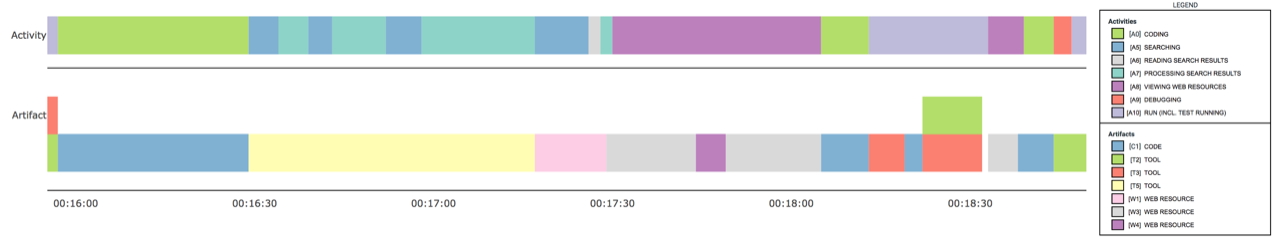
\includegraphics[width=1.98\columnwidth]{figures/P6timeplot}
\caption{Snippet of Activities and Artifacts from P6 (real-world IDE development, 5-minute duration)}
\label{P6Fig}
\end{figure*}


\begin{figure}
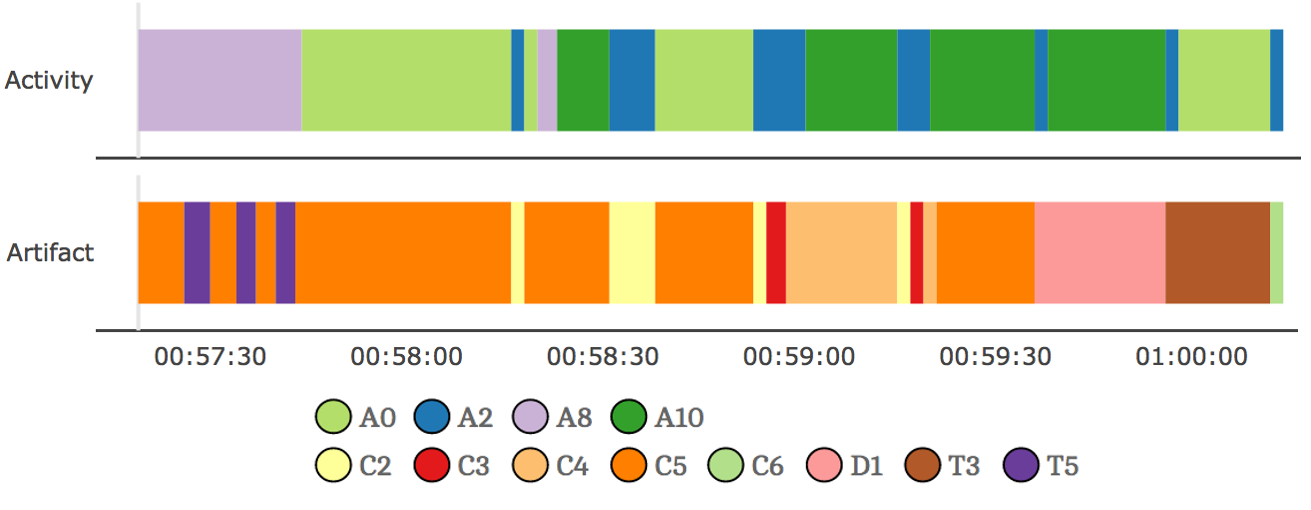
\includegraphics[width=\columnwidth]{figures/P4timeplot}
\caption{Snippet of Activities and Artifacts from P4 (traffic intersection prompt, 3-minute duration)}
\label{P4Fig}
\end{figure}
\boldification{**based on the activity, the interaction with artifacts change**}

When participants access the artifacts, the specific interactions with the artifacts -- selecting which part of the artifact to go to, whether they simply scroll through the artifact or highlight parts of the artifact, whether they copy text from these artifacts to paste into the code for debugging -- depends on the programming activity and the goal driving the activity. These differences are also observable through the difference in times spent on these artifacts.

Figure~\ref{P6Fig} shows the artifacts P6 accesses and the activities he performs. A marks the time P6 searched on the web to obtain the syntax for a java script feature. The first time he reaches a Q and A web page containing answers to his question (marked B) on the diagram, he scrolls through the first few answers before selecting one spending around 36 seconds. These interactions was driven by the goal to learn how to implement the feature for the purpose of coding [A0]. When his selected answer threw an error (marked as C), he went back to the web page and quickly scrolled and found the answer he had already identified (marked as D) and copies it to implement. This second visit to the web page took only five seconds and was geared towards recalling the syntax for debugging purposes [A9]. 

Brandt et. al.~\cite{Brandt:2009} observed similar behavior in programmers where he was able to distinguish between the purposes of when programmers use online resources. He also found that participants spent the most time when learning from the web and least time when using the web to recall syntax.

\boldification{**memory plays a role - sequence matters [same activity, shorter time, memory plays role] [zoomed out figure]}

We also observe that memory plays a role in the interaction with artifacts. In the above example, across the different the coding [A0] and debugging [A9] activities, when P6 visited the web page a second time it took him exactly five seconds to locate the syntax and copy it. We infer that he could recall from his memory where the desired information was located. We observe such a mapping between information and artifacts were referred to by the participants repeatedly. This mapping was influenced by the programming activities and the goal behind the activities.

\boldification{**Not only does context rise from the activity i.e. activity guides the specific type and amount of information obtained from the context/artifact, the activity was used to recall the relation between the context with which the artifacts were associated**}

Thus, we see that not only does context rise from the activity, the programming activity and the goal behind it guides the specific type and amount of information obtained from the artifact that comprises the context. The programming activity is used to recall the relation between the information and the artifacts within the context.


\boldification{**this means that?.and is contrary to the assumptions of ?representational view of context, that context is stable and separate from activities? [...], is not what we see in our data. }

\subsection{Interaction includes Reflection}

\boldification{**Finally we see that, users conduct reflection/evaluation of the information they come across before deciding their next activity**}

Participants continuously performed evaluation of the information within an artifact and followed up with reflecting upon the information they used towards the solution. We observe these evaluation sessions through interactions that prolong the participant's current activity---long scrolls, reading the artifact multiple times etc. When participants hit a wall, they often went back to 



Most of the times, the first attempt never leads to 

When interacting with artifacts, participants continuously performed reflection and evaluation of the information before moving to the next programming activity. For example, P1 tried to implement his idea using `case classes' in scala in the code file c3. When trying to define these `case classes' his IDE declared errors. He spent 20 seconds trying to fix the error and reflecting on his prior experiences. He said ``I don't know how to do this'' and so visited the documentation web page w5 and spent 24 seconds reading and scrolling. P1 made some evaluation of the information and effort needed to implement `case class', and decided to ``\dots do it smartly'' and ``\dots just do it with strings''.

Figure \ref{P4Sketch}

\begin{figure}
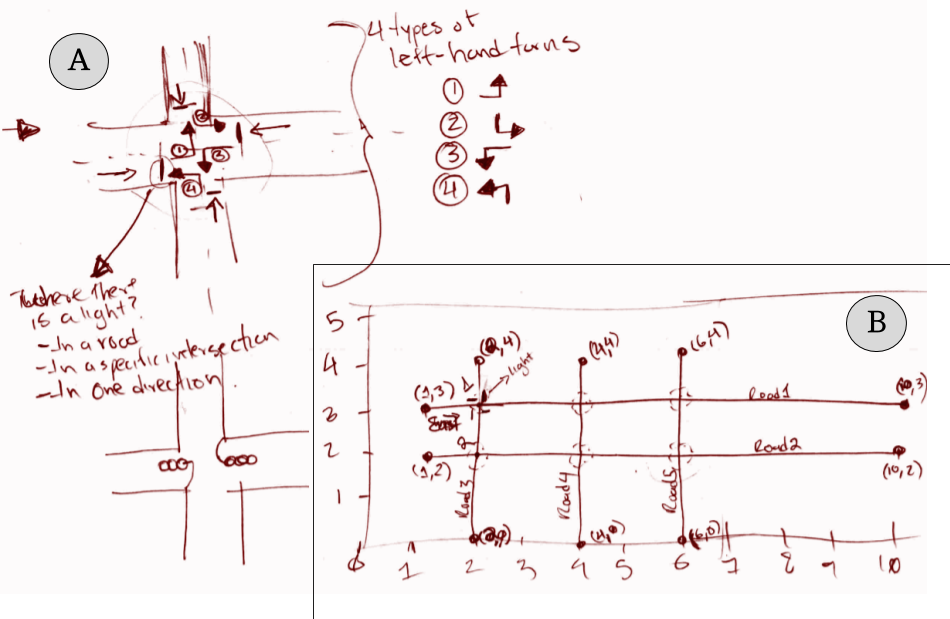
\includegraphics[width=\columnwidth]{figures/P4sketches}
\caption{External artifacts created by P1 during the session}
\label{P4Sketch}
\end{figure}

We conclude from all our observations that along with the \textit{representational} and \textit{interactional} components of context, there exists an informational component. Participants looked for different types of information and consumed different amounts of information from various representations that have been known to affect context viz. time, environment etc. The various interactions determined how information was consumed by the participants. 
%!TEX root = main.tex

\section{Discussion and Future Directions}
\textbf{Limitations:} Like any research our study has limitations. First, this was an exploratory study that only included six participants recruited through convenience sampling. All participants had at least five years of programming experience, with three participants having three or more years of professional programming experience. Second, we collected different types of data across the participants-- screen sharing was captured for all participants, but P4 included video of the participants face during the study and P1 provided think-aloud audio. Since our primary goal was to observe the interactions between participants and the artifacts they utilized during programming, screen capture data was the primary focus during our studies. The observations we discuss in this paper are from the preliminary analysis of data we collected to understand the role of context in programming.

%Based on this data, our analysis focused on the actions we could observe in screen capture data, which we validated with the available audio, video, and external documents (such as notes on the provided paper).

 Like many other research papers based on formative analysis, our observations  are subject to threats to validity. We chose our participants through convenient sampling and observed participants through online mediums as well as physical mediums. But our focus was to understand how context is created---how artifacts are used, how information is evaluated and mapped to the problem to be solved, and how programming activity guides the interaction with the artifacts. The \emph{``problem is not that context does not matter; it matters a great deal''}~\cite{Dourish:2004}, the problem is defining and operationalizing what context is. Hence, it was more important to observe these patterns of interactions and activities than restrict the medium and people we observe these patterns through.

%\subsection{Future Directions}
Based on our initial anal
Our initial analysis reveals two future directions that we plan to pursue. 

\boldification{**Goal: apply IFT to create a model of how the context that is created and recommend artifacts for the context for a given programming activity}

\textit{Using Information Foraging Theory to inform context creation:}
Context has been largely defined as all `relevant information' that an individual needs to complete a task. We believe that Information Foraging Theory (IFT) constructs~\cite{Pirolli:1995,Fleming:2013} can help us model how programmers find information in an artifact and decide whether it is relevant as they carry out their tasks. IFT explains that the consumption of information is similar to how animals hunt for food---following scent of their prey and choosing more valuable prey through a cost-benefit analysis. We observed that participants engaged in such evaluation of artifacts and the information contained within when building context. 

% Although context is ``hard to elucidate''~\cite{Abowd:1999}, time and again researchers claim that context is `relevant information'. Due to this informational nature, and from our observations, the creation of context sits well with Information Foraging Theory(IFT) constructs~\cite{Pirolli:1995,Fleming:2013}. IFT explains that consumption of information is similar to how animals hunt for food---following scent and choosing more valuable preys. We observed that participants engaged in reflection and evaluation of information hen creating and using context. 

IFT has been applied in the programming domain to study how varying goals~\cite{Piorkowski:2015} affect the perceived value of information and how the (perceived) cost of `consuming' information varies across different types of artifacts (e.g., web site vs. Q\&A forum) ~\cite{Jin:2017}. We plan to build on these works to explore how IFT can help model programmers context building behavior. 

%We plan to explore the application of Information Foraging Theory (IFT)~\cite{Jin:2017,Fleming:2013} to model how context is created during programming, and to develop recommendations of artifacts that are relevant to a given programmer and a programming activity. IFT is applicable to programmer context since information seeking and cost-benefit analysis are central concerns when examining an artifact for usefulness (or value) to the overarching context of a programming activity.


\boldification{More work is needed on:
**Mapping
**sense-making of the information to see if it fits in the context also while alluded has not been really operationalized and is needed for future studies
**memory modeling
**How people recall information, and map information to a context has also not been looked at
**recall- memory has not been explicitly looked at in the IFT MODEL..recency has been used for predicting behavior, something that needs more investigation
**externalizing/ enriching information patches
**This selection of information based on the already existing context is similar to that pointed out in the IFT Domain. Obtaining and processing information has cost associated with it. The cost varies from having to open and process and new page to just recalling information already existing in the context**}

\subsubsection{Mapping and Memory Modeling}
Our observations show that participants accessed artifacts and reflected on the information contained in them. Past work has alluded to how individuals perform ``sensemaking'' of information contained withing artifacts to fit their (task) goal ~\cite{Grigoreanu:2012}, but the process by which individuals map the information they find to the problem or solution space has not been modeled. Moreover, once a context has been built parts of the context (information) can be useful and recalled from memory for another (programming) task. Further studies are needed to understand how individuals recall snippets of context from other tasks to aid their current one or how temporality of actions may cause decay in memory and the ability to recall context.

% Our observations show that participants continuously make sense of the information to build context. The process of making sense of information contained within artifacts to determine a fit within a particular context has been alluded to in previous work~\cite{Pirolli:2005,Grigoreanu:2012}, but has not been examined from operationalization perspective. Once a context is built, information is recalled form the memory. This information may be from a different context, in which case the applicability of information in a different context has to be re-evaluated.


% }
% \subsubsection{Scope for Further work:}
% \begin{itemize}[leftmargin=6pt, parsep=0pt, topsep=0pt]
% \item \textbf{Mapping}: Examining the mapping between artifacts and context. The process of making sense of information contained within artifacts to determine a fit within a particular context has been alluded to in previous work~\cite{Pirolli:2005}, but has not been examined from operationalization perspective.
% \item \textbf{Memory Models}: Modeling the ways in which programmers recall information and map that information to a particular context. Memory has been examined in the IFT model for predicting information-seeking behavior~\cite{Lawrance:2010,Lawrance:2013}, but there is further work needed to investigate the effects of context.
% \item \textbf{Externalizing/Enriching Information Patches}: Also examined in the domain of IFT, the selection of information based upon the already existing context incurs a cost. Information costs are associated with the effort required to obtain it, but determining whether that information previously existed in context and can simply be recalled has not been explored.
% \end{itemize}

\bibliographystyle{ACM-Reference-Format}
\bibliography{bibliography} 

\end{document}
